\section{Java Persistence API}
An application permits the management of the bill of materials (BoM) of products. The BoM is the hierarchical description of a product in terms of the 
sub-products that comprise it. At each level but the last one, a product is associated with the components that make it, each with a quantity. The application 
allows the user to create BoMs. A BoM is progressively assembled by attaching to a product its sub-products and specifying the number of units of sub-products 
that make one unit of the parent product. The editor accesses the HOME PAGE with the list of current BoMs and where s/he can create a new top level product and 
view the existing BOMs. The editor can add product-sub-products links to a product, modify the quantity of a product-sub-products link, delete a product or
product-sub-products link. Products have an identifier, a name a description and a unit cost. An example of BoM is the following: 
\begin{figure}[H]
    \centering
    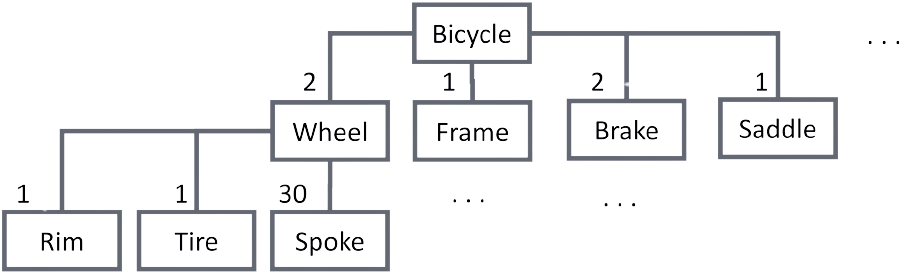
\includegraphics[width=0.6\linewidth]{images/BoM.png}
\end{figure}
The entity relationship model is the following:
\begin{figure}[H]
    \centering
    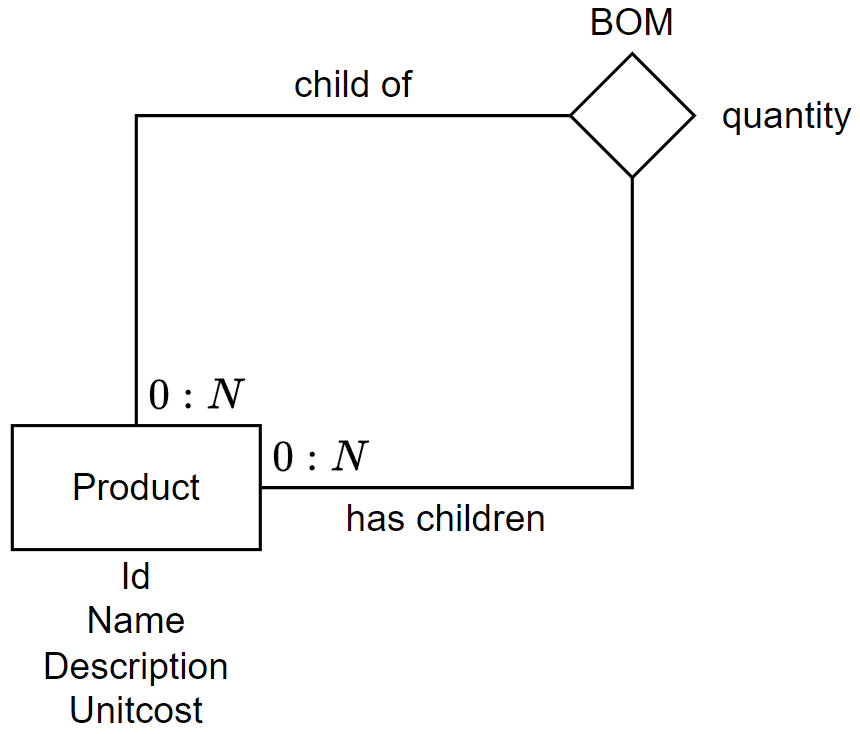
\includegraphics[width=0.3\linewidth]{images/e-r1.png}
\end{figure}
The relational schema DDL of the given database is: 
\begin{lstlisting}[style=SQL]
CREATE TABLE 'product' (
'id'            INT             NOT NULL AUTO_INCREMENT,
'unitcost'      INT             NOT NULL,
'name'          VARCHAR(45)     NOT NULL,
'description'   VARCHAR(45)     DEFAULT NULL,
PRIMARY KEY ('id')
) 
CREATE TABLE 'subparts' (
'father'        INT             NOT NULL,
'child'         INT             NOT NULL,
'quantity'      INT             NOT NULL,
PRIMARY KEY ('father','child'),
KEY 'childtoproduct_idx' ('child'),
CONSTRAINT 'childtoproduct' FOREIGN KEY ('child') REFERENCES 'product' ('id'),
CONSTRAINT 'fathertoproduct' FOREIGN KEY ('father') REFERENCES 'product' ('id')
)           
\end{lstlisting}
The relational model is: 
\begin{itemize}
    \item Product(\underline{id}, unitcost, name, description)
    \item Subparts(\underline{father}, \underline{child}, quantity)
\end{itemize}
Given the specifications, write the entity classes of the ORM mapping, including annotations for the attributes and for the relationships, fetch type of 
attributes and of relationships, and operation cascading policies for relationships (when not by default).

\paragraph*{Solution}
Given the specifications write the entity classes of the ORM mapping, including annotations for the attributes and for the relationships, fetch type of attributes
and of relationships, and operation cascading policies for relationships (when not by default). 

\begin{itemize}
    \item BoM: from father product to children product we have to use the annotations: 
        \begin{lstlisting}[style=Java]
@ManyToMany
        \end{lstlisting}
        From children product to father product we have to use these annotations: 
        \begin{lstlisting}[style=Java]
@ManyToMany
        \end{lstlisting}
        The owner of the relation is entity project. 
    \item 
\end{itemize}
The entity product is defined as:  
    \begin{lstlisting}[style=Java]
@Entity
@NamedQueries({
@NamedQuery(name = "BomProduct.findAll", query = "SELECT p FROM BomProduct p"),
@NamedQuery(name = "BomProduct.findAllTop", query = "SELECT p FROM BomProduct p WHERE p.fathers IS EMPTY") })

public class BomProduct implements Serializable {
    ...
    private static final long serialVersionUID = 1L;
    @Id @Column(name="id") @GeneratedValue(strategy = GenerationType.IDENTITY)
    private int id;
    private String description;
    private String name;
    private int unitcost;
    ...
    @ElementCollection(fetch = FetchType.EAGER)
    @CollectionTable(name = "subparts",joinColumns = @JoinColumn(name = "father"))
    @MapKeyJoinColumn(name = "child")
    @Column(name = "QUANTITY")
    private Map<BomProduct, Integer> subparts;

    @ManyToMany
    @JoinTable(name = "subparts",
            joinColumns = @JoinColumn(name = "child"),
            inverseJoinColumns = @JoinColumn(name ="father"))
    private List<BomProduct> fathers;
    ...            
}
    \end{lstlisting}
The better way is to make the many-to-many relationships with attributes a weak entity like in the following image. 
\begin{figure}[H]
    \centering
    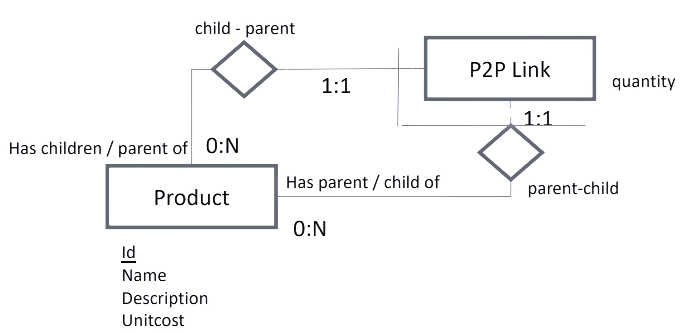
\includegraphics[width=0.5\linewidth]{images/BoMweak.png}
\end{figure}
The entity P2PLinkID is defined as:  
\begin{lstlisting}[style=Java]
@Embeddable
public class P2PLinkID implements Serializable {
    private static final long serialVersionUID = 1L;
    private int father;
    private int child;

    public P2PLinkID() { }

    public P2PLinkID(int father, int child) {
        super();
        this.father = father;
        this.child = child;
    }
    ...
}
\end{lstlisting}
The entity P2PLink is defined as:  
\begin{lstlisting}[style=Java]
@Entity
public class P2PLink implements Serializable {
    private static final long serialVersionUID = 1L;

    @EmbeddedId
    private P2PLinkID id;

    @ManyToOne
    @MapsId("father") // reference to the foreign key attribute
    @JoinColumn(name = "father")
    private BomProduct father;

    @ManyToOne
    @MapsId("child") // reference to the foreign key attribute
    @JoinColumn(name = "child")
    private BomProduct child;

    private int quantity;
    ...
}
\end{lstlisting}
The entity product is defined as:  
\begin{lstlisting}[style=Java]
@Entity
public class BomProduct implements Serializable {
    private static final long serialVersionUID = 1L;

    @Id @GeneratedValue(strategy = GenerationType.IDENTITY)
    private int id;
    private String description;
    private String name;
    private int unitcost;

    // getters setters and constructors

    @OneToMany(mappedby="father")
    private List<P2PLink> children;

    @OneToMany(mappedby="child")
    private List<P2PLink> fathers;
    ...
}
\end{lstlisting}